\begin{frame}[label=mc_results]
    \frametitle{Results: Bistatic Link Performance}
    \begin{columns}
        \begin{column}{0.75\textwidth}
            \textit{Starting basic:} 
            
            Investigating a single link at increasing \textcolor{blue}{\textbf{TX}}-\textcolor{red}{\textbf{RX}} distances
            {\begin{itemize}
                \footnotesize %
                \item \alert{Similar performance at 0-50 km separation}
                \item Steady degradation of counts and density at 50+ km
            \end{itemize}} %
            \centering %
            \begin{tikzpicture}
                \node[inner sep = 0, anchor=south] (img) { 
                    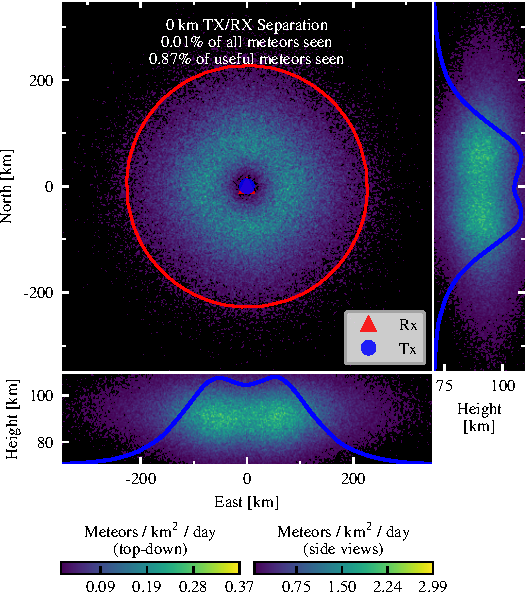
\includegraphics[height=0.38\textheight]{img/simulated_heatmap_0km.pdf}
                };
                \node[anchor=south, inner sep = 0] at ([yshift = -0.0cm, xshift=-0.2cm]img.north) { 
                     \tiny \colorbox{yellow}{0 km}
                };
                \node[inner sep = 0, anchor=west] (img2) at (img.east) { 
                    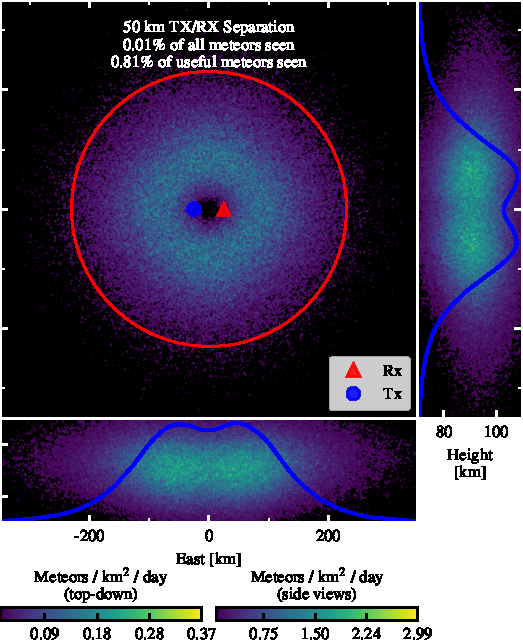
\includegraphics[height=0.38\textheight]{img/simulated_heatmap_50km.pdf}
                };
                \node[anchor=south, inner sep = 0] at ([yshift = -0.0cm, xshift=-0.2cm]img2.north) { 
                    \tiny \colorbox{yellow}{50 km}
                };
                \node[inner sep = 0, anchor=west] (img3) at (img2.east) { 
                    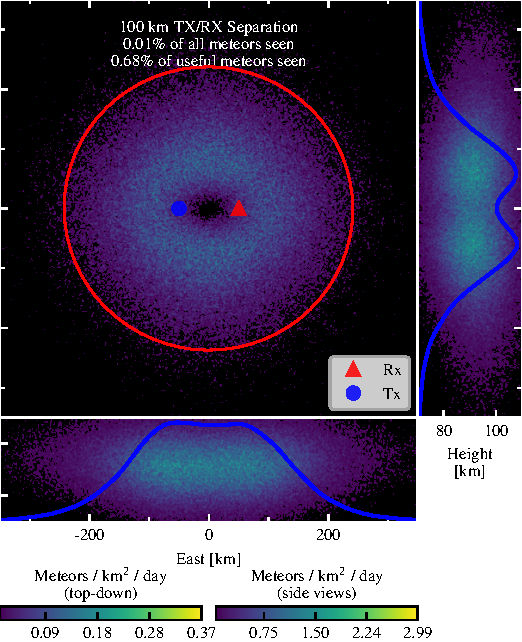
\includegraphics[height=0.38\textheight]{img/simulated_heatmap_100km.pdf}
                };
                \node[anchor=south, inner sep = 0] at ([yshift = -0.0cm, xshift=-0.2cm]img3.north) { 
                    \tiny \colorbox{yellow}{100 km}
                };
                \node[inner sep = 0, anchor=west] (img4) at (img3.east) { 
                    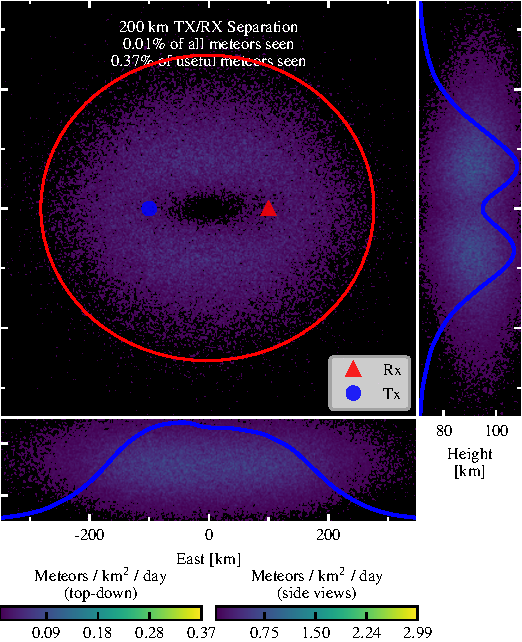
\includegraphics[height=0.38\textheight]{img/simulated_heatmap_200km.pdf}
                };
                \node[anchor=south, inner sep = 0] at ([yshift = -0.0cm, xshift=-0.2cm]img4.north) { 
                    \tiny \colorbox{yellow}{200 km}
                };
            \end{tikzpicture}
        \end{column}
        \begin{column}{0.3\textwidth}
            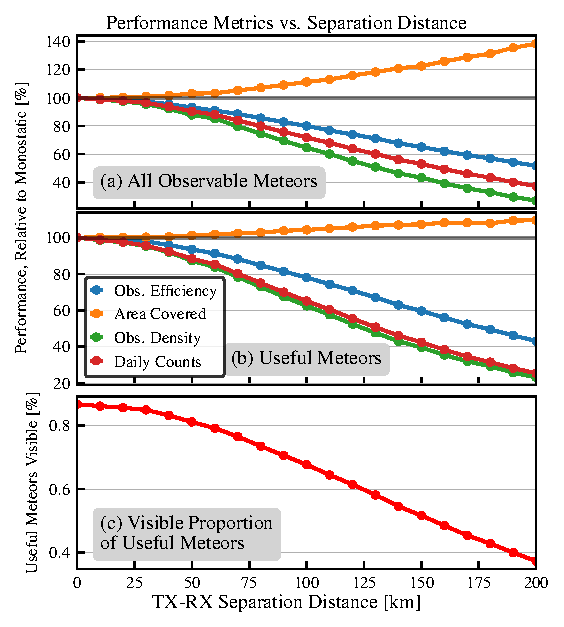
\includegraphics[width=\linewidth]{img/sim_analysis.pdf}
        \end{column}
    \end{columns}
    \centering
\end{frame}